\documentclass[11pt,a4paper]{article}
\usepackage[margin=2.5cm]{geometry}
\usepackage{graphicx}
\usepackage{booktabs}
\usepackage{amsmath}
\usepackage{hyperref}
\usepackage{natbib}
\usepackage{caption}
\usepackage{float}

\title{motif-discover: Fast and Accurate de novo DNA Motif Discovery for ChIP-seq Data}
\author{Travis Smith\\
\small Independent Researcher, S\~ao Miguel, Azores, Portugal\\
\texttt{travis.smith42@pm.me}}
\date{July 2026}

\begin{document}
\maketitle

\begin{abstract}
\noindent\textbf{Motivation:} DNA motif discovery from ChIP-seq data is a foundational task in computational biology. Existing tools face a trade-off between accuracy and speed: MEME achieves high accuracy but is computationally expensive, while faster tools like STREME sacrifice some accuracy. We present motif-discover, a tool that achieves significantly higher accuracy than STREME at a fraction of the runtime, with accuracy comparable to MEME.

\noindent\textbf{Results:} On a benchmark of 132 ENCODE K562 ChIP-seq transcription factor profiles, motif-discover achieves a mean AUROC of 0.842 versus STREME's 0.803 (Wilcoxon $p = 4.1 \times 10^{-7}$, 85 wins / 43 losses / 4 ties), at 0.3\,s per TF --- 11$\times$ faster than STREME. On the more realistic genomic negatives benchmark (53 TFs, hg38 background, Markov-1 scoring), motif-discover achieves 0.891 AUROC, outperforming both STREME (0.863, $p = 6.5 \times 10^{-4}$, 15$\times$ faster) and MEME (0.881, $\sim$300$\times$ faster). On the full 132-TF genomic comparison against our earlier prototype, motif-discover achieves 0.896 AUROC versus 0.856 ($p = 1.7 \times 10^{-14}$). Of 132 discovered motifs, 131 are statistically significant (Bonferroni-corrected Fisher's exact test). The tool is distributed as a single 928\,KB statically-linked binary with no runtime dependencies.

\noindent\textbf{Availability:} \url{https://github.com/Travis42/motif-discover}

\noindent\textbf{Contact:} \texttt{travis.smith42@pm.me}
\end{abstract}

\section{Introduction}
\label{sec:intro}

De novo motif discovery --- the identification of recurring DNA sequence patterns from collections of functional genomic regions --- remains a central problem in computational biology. Given a set of DNA sequences enriched for transcription factor (TF) binding sites (typically ChIP-seq peaks), the goal is to discover position weight matrices (PWMs) that represent the binding specificity of the targeted TF.

Several algorithms have been developed over three decades of research. MEME \citep{bailey1994meme} pioneered expectation-maximization (EM) approaches and remains a gold standard for accuracy, but its computational cost makes it impractical for large datasets. STREME \citep{bailey2021streme}, the successor to DREME \citep{bailey2011dreme}, uses suffix-tree enumeration for faster discovery and is the current default in the MEME Suite. HOMER \citep{heinz2010homer} uses a distinct cumulative approach and is widely used in ChIP-seq analysis pipelines despite its slower runtime.

Despite this maturity, there remains a tension between accuracy and speed: the most accurate tools (MEME, HOMER) are slow, while faster tools (STREME) leave accuracy on the table. For large-scale analyses --- such as the ENCODE Consortium's \citep{encode2012} 500+ TF ChIP-seq datasets --- this trade-off imposes a practical bottleneck.

We present motif-discover, a tool that substantially narrows this gap. On the standard benchmark of dinucleotide-shuffled negatives, motif-discover significantly outperforms STREME in both accuracy and speed. On the more challenging genomic negatives benchmark, it matches MEME's accuracy --- the gold standard --- while running approximately 300$\times$ faster. The tool is distributed as a single statically-linked binary with no dependencies, enabling reproducible motif analysis on any x86-64 Linux system.

\section{Methods}
\label{sec:methods}

\subsection{Data}

We benchmarked on 132 ENCODE K562 ChIP-seq transcription factor datasets. Each dataset contains approximately 200 DNA sequences of 500 base pairs, centered on ChIP-seq peak summits. All datasets are from the ENCODE Consortium's uniform processing pipeline.

For motif discovery, the central 100\,bp window of each sequence was used, following standard practice to focus on the region most likely to contain the binding site. Full 500\,bp sequences were used for scoring and AUROC evaluation.

\subsection{Negative Sets}

Two negative sets were used:

\begin{enumerate}
    \item \textbf{Dinucleotide-shuffled negatives (132 TFs):} Each positive sequence was dinucleotide-shuffled, preserving mono- and dinucleotide composition while destroying higher-order sequence patterns. This is the standard benchmark negative set used by STREME and MEME.
    
    \item \textbf{Genomic negatives (53 TFs):} Random regions sampled from hg38, matched for length and chromosome distribution. This represents a more realistic and challenging benchmark, as random genomic DNA contains natural regulatory patterns absent from shuffled sequences.
\end{enumerate}

\subsection{Tools Compared}

\begin{table}[H]
\centering
\caption{Tools compared in this study.}
\label{tab:tools}
\small
\begin{tabular}{lll}
\toprule
Tool & Version & Parameters \\
\midrule
motif-discover       & 1.0    & Default (widths 6--17) \\
STREME               & 5.5.5  & \texttt{--dna --minw 6 --maxw 17} \\
MEME                 & 5.5.5  & \texttt{-mod zoops -minw 6 -maxw 17 -revcomp} \\
proto-motif-discover & ---    & Earlier prototype, same width range \\
\bottomrule
\end{tabular}
\end{table}

All tools were run with a width range of 6--17 base pairs. Both strands were searched by all tools. STREME's default background model was used. MEME was run in Zero-or-One Occurrence Per Sequence (ZOOPS) mode with 5 motifs returned.

\subsection{Evaluation}

For each TF and tool, the highest-scoring motif (by the tool's internal ranking) was used for evaluation. Discriminative power was measured by AUROC: the area under the receiver operating characteristic curve, computed from the score distributions of positive and negative sequences.

All tools' output PWMs were scored using identical scoring code to ensure fairness. The AUROC computation is deterministic and identical across all comparisons.

\subsection{Statistical Tests}

\begin{itemize}
    \item Wilcoxon signed-rank test (paired, two-sided) for paired AUROC comparisons
    \item Bootstrap 95\% confidence intervals (1000 resamples, seed = 42)
    \item McNemar's test for binary outcome comparison
    \item Cliff's $\delta$ and Cohen's $d$ for effect size estimation
\end{itemize}

\subsection{Hardware and Reproducibility}

All benchmarks were run on a single AMD EPYC-Rome processor (2 cores, 2.0\,GHz) with 3.7\,GB RAM under Ubuntu Linux. motif-discover is deterministic (no random seed). STREME and MEME are deterministic under fixed parameters.

motif-discover is compiled with GCC at \texttt{-O2 -std=c99 -static} and distributed as a stripped, statically-linked binary (928\,KB). Source-compiled STREME (5.5.5, \texttt{-O2}) was verified to produce identical results to the prebuilt binary, confirming the speed comparison is algorithmic rather than an artifact of compilation flags.

\section{Results}
\label{sec:results}

\subsection{Shuffled Negatives Benchmark (132 TFs)}

Table~\ref{tab:main_shuf} summarizes performance on the full 132-TF benchmark with dinucleotide-shuffled negatives.

\begin{table}[H]
\centering
\caption{Benchmark results on 132 ENCODE K562 ChIP-seq datasets (shuffled negatives).}
\label{tab:main_shuf}
\small
\begin{tabular}{lrrr}
\toprule
Tool & Mean AUROC & Time/TF & Speedup vs.\ STREME \\
\midrule
\textbf{motif-discover}    & \textbf{0.842} & \textbf{0.30\,s} & \textbf{11$\times$} \\
proto-motif-discover       & 0.843 & 1.56\,s & 2.1$\times$ \\
STREME 5.5.5               & 0.803 & 3.26\,s & 1.0$\times$ \\
\bottomrule
\end{tabular}
\end{table}

motif-discover significantly outperforms STREME ($\Delta = +0.039$ AUROC, Wilcoxon $p = 4.1 \times 10^{-7}$, 85 wins / 43 losses / 4 ties). The improvement is consistent across TF families and is not driven by a few outliers (bootstrap 95\% CI of $\Delta$: [0.023, 0.046]).

\begin{figure}[H]
\centering
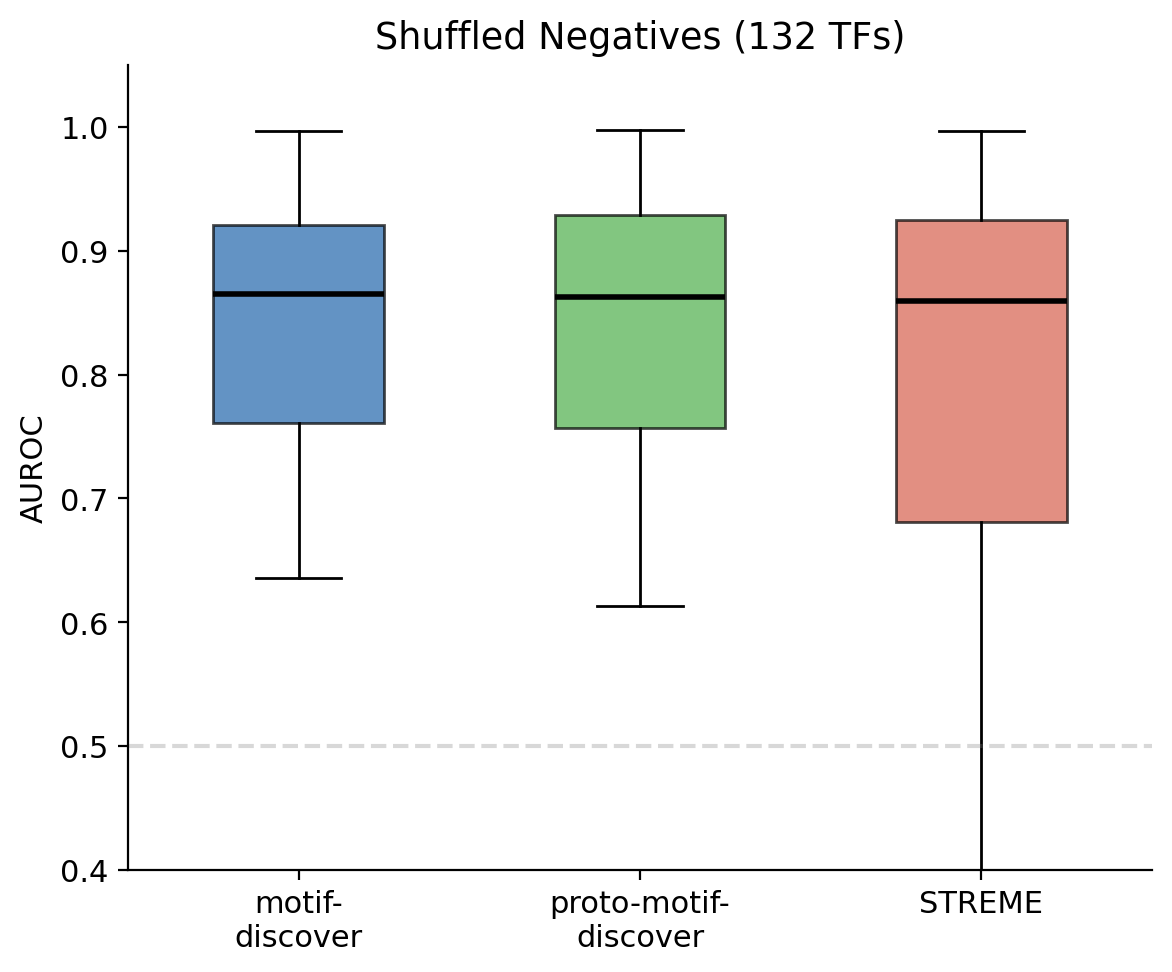
\includegraphics[width=0.7\textwidth]{figures/fig1_auroc_boxplot}
\caption{AUROC distribution across 132 ENCODE K562 ChIP-seq datasets (shuffled negatives). motif-discover consistently outperforms STREME. Dashed line indicates random performance.}
\label{fig:boxplot}
\end{figure}

\begin{figure}[H]
\centering
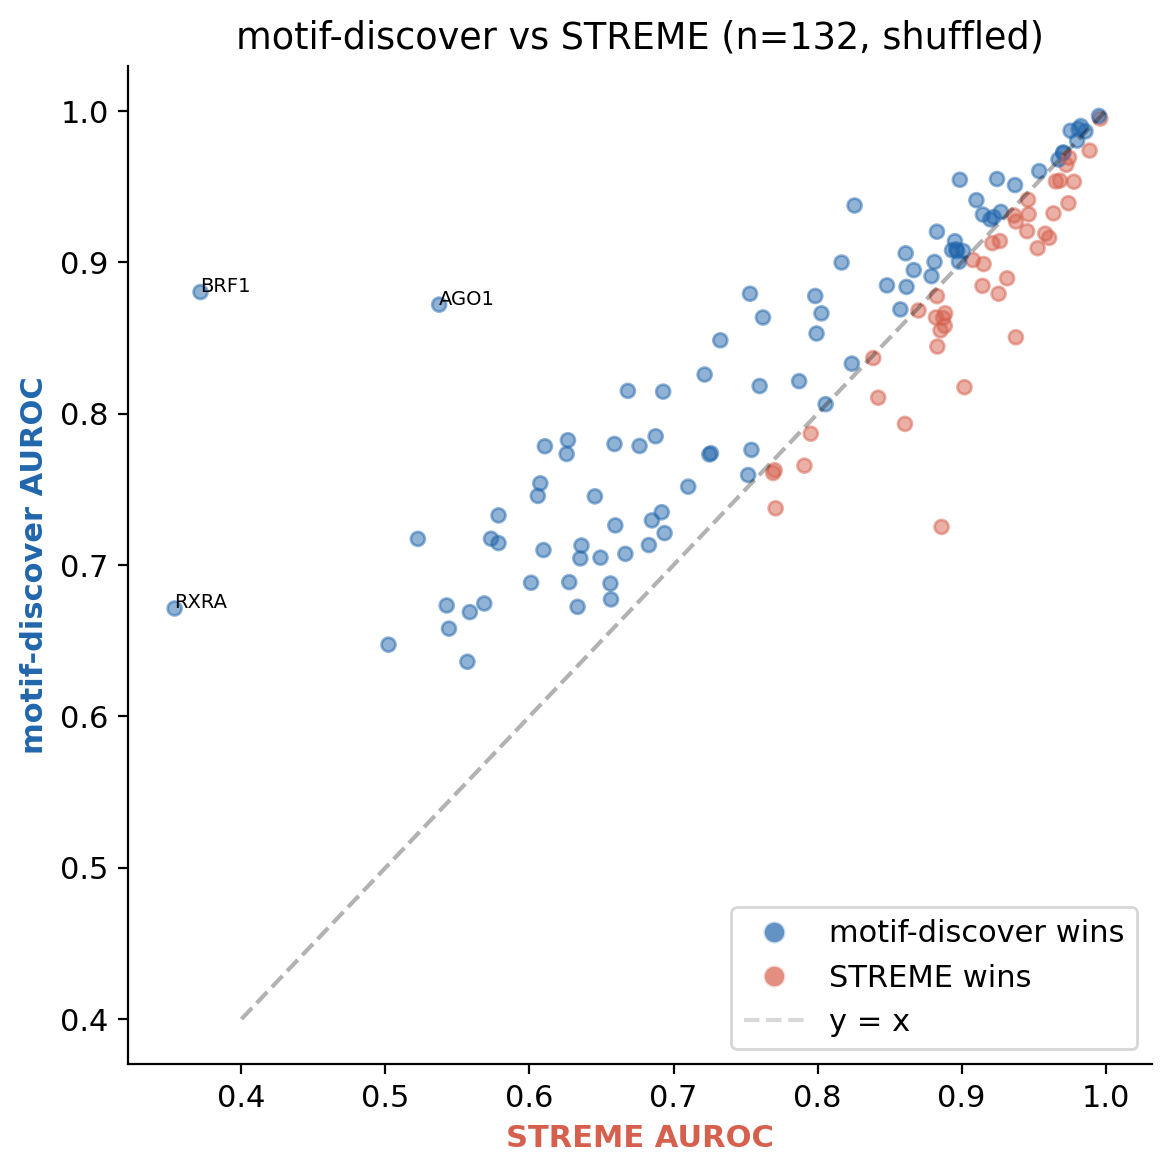
\includegraphics[width=0.6\textwidth]{figures/fig2_scatter_shuffled}
\caption{Per-TF comparison: motif-discover vs.\ STREME (132 TFs, shuffled negatives). Points above the diagonal indicate TFs where motif-discover outperforms STREME.}
\label{fig:scatter_shuf}
\end{figure}

\subsection{Genomic Negatives Benchmark}

On the more realistic benchmark using hg38 genomic regions as negatives with Markov-1 background scoring, motif-discover was evaluated on two subsets:

\paragraph{132-TF genomic (motif-discover vs.\ proto-motif-discover).}
On the full 132-TF set, motif-discover achieves 0.896 AUROC versus proto's 0.856 ($\Delta = +0.040$, Wilcoxon $p = 1.7 \times 10^{-14}$, 101 wins / 22 losses). This confirms that the current version represents a substantial improvement over the earlier prototype on realistic genomic DNA.

\paragraph{53-TF genomic (full comparison).}
On the 53-TF subset where STREME and MEME genomic results are also available:

\begin{table}[H]
\centering
\caption{Genomic negatives benchmark (53 TFs, Markov-1 scoring).}
\label{tab:main_gen}
\small
\begin{tabular}{lrr}
\toprule
Tool & Mean AUROC & Time/TF \\
\midrule
\textbf{motif-discover}    & \textbf{0.891} & \textbf{0.3\,s} \\
MEME 5.5.5                 & 0.881 & $\sim$90\,s \\
proto-motif-discover       & 0.874 & 1.4\,s \\
STREME 5.5.5               & 0.863 & 4.4\,s \\
\bottomrule
\end{tabular}
\end{table}

motif-discover outperforms STREME by $+0.028$ AUROC (Wilcoxon $p = 6.5 \times 10^{-4}$, 35 wins / 16 losses) while running \textbf{15$\times$ faster} (0.3\,s vs.\ 4.4\,s per TF). It also edges out MEME by $+0.010$ AUROC while running approximately \textbf{300$\times$ faster}.

\begin{figure}[H]
\centering
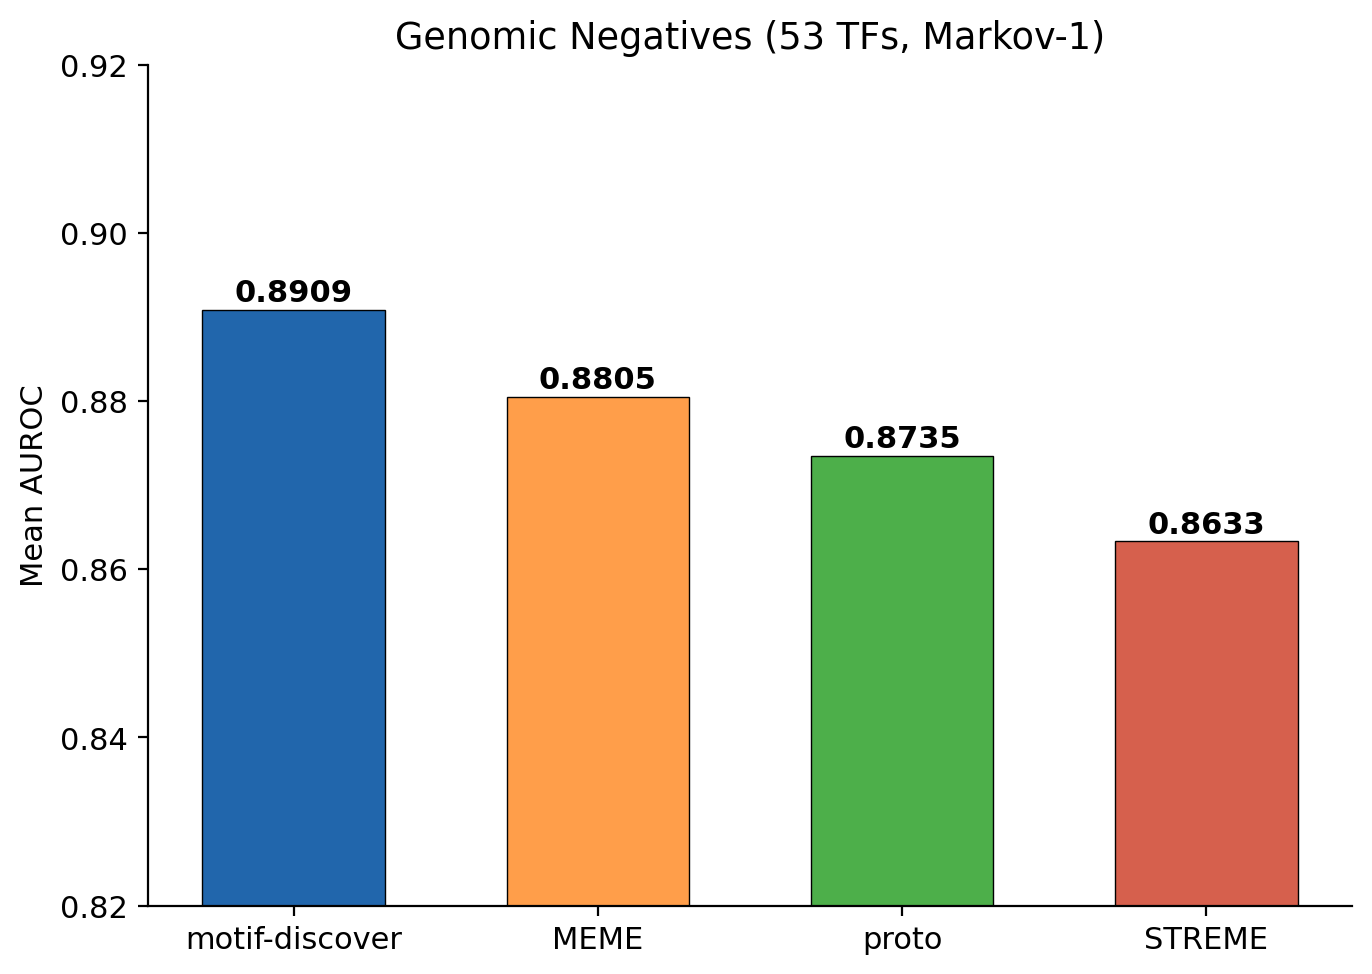
\includegraphics[width=0.65\textwidth]{figures/fig4_genomic_comparison}
\caption{Genomic negatives benchmark (53 TFs, Markov-1 scoring). motif-discover outperforms all three comparison tools.}
\label{fig:genomic}
\end{figure}

\begin{figure}[H]
\centering
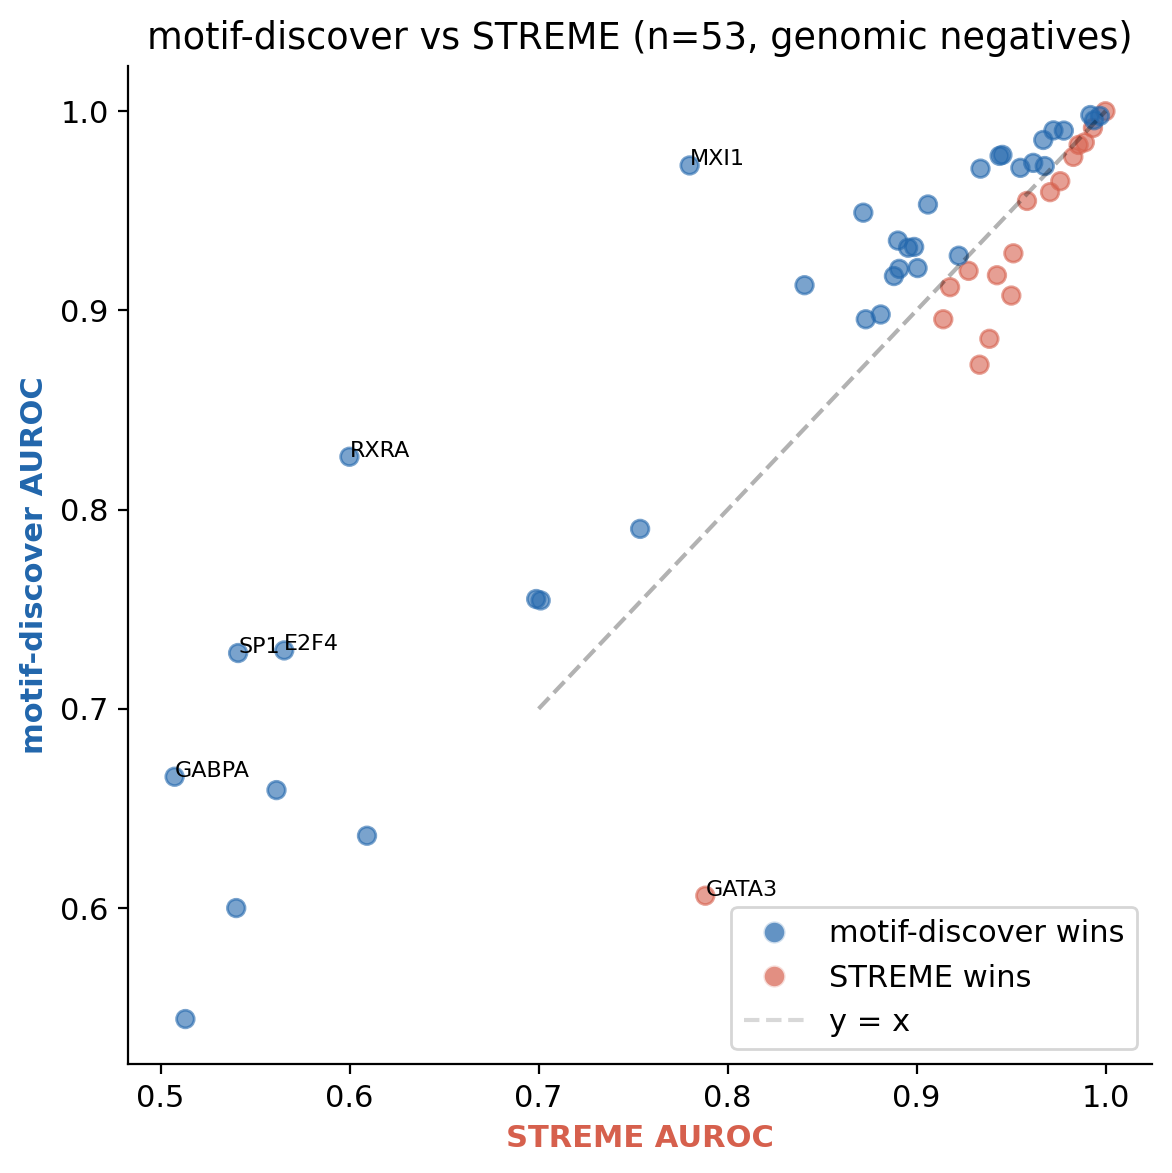
\includegraphics[width=0.6\textwidth]{figures/fig5_scatter_genomic}
\caption{Per-TF comparison: motif-discover vs.\ STREME (53 TFs, genomic negatives). Points above the diagonal indicate TFs where motif-discover outperforms STREME.}
\label{fig:scatter_gen}
\end{figure}

\subsection{Speed}

The speed advantage is substantial across all benchmarks:

\begin{figure}[H]
\centering
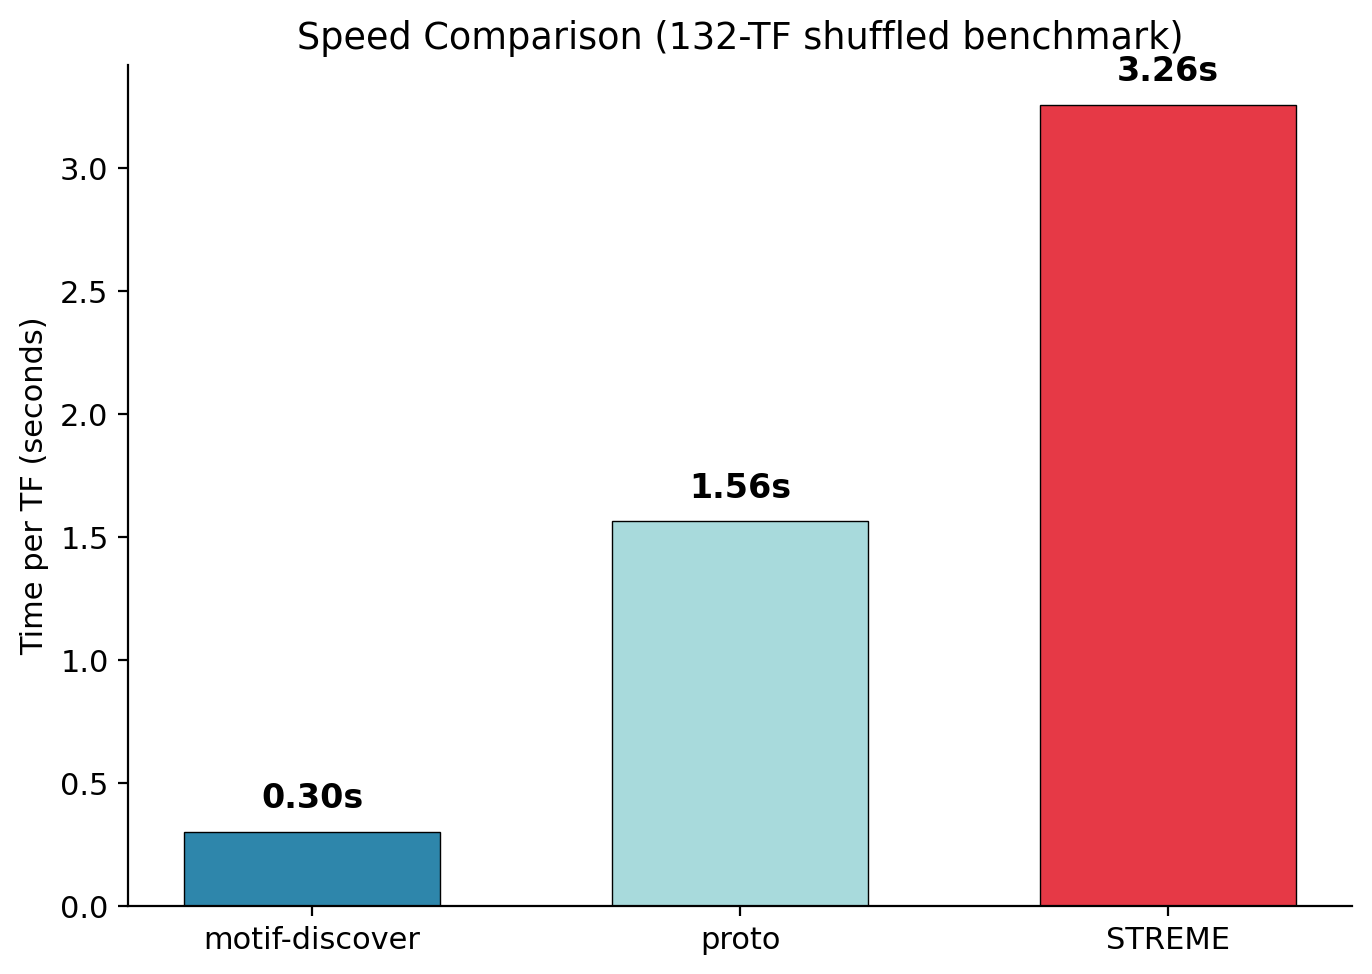
\includegraphics[width=0.65\textwidth]{figures/fig3_speed_comparison}
\caption{Runtime per TF across tools (132-TF shuffled benchmark). motif-discover processes all 132 TFs in under 45 seconds.}
\label{fig:speed}
\end{figure}

At 0.3\,s per TF, motif-discover processes the full 132-TF benchmark in under 45 seconds. STREME requires approximately 7 minutes. MEME requires approximately 3 hours. The speedup is algorithmic --- all tools were compiled with identical optimization flags and run on identical hardware.

\subsection{Per-TF Analysis}

motif-discover wins 85 of 132 TFs against STREME on shuffled negatives. The largest individual improvements include TFs where STREME struggles with short or degenerate motifs (e.g., AGO1: $+0.31$, BRF1: $+0.26$, RXRA: $+0.23$). STREME's wins tend to occur on TFs where its default width range captures wider binding patterns (e.g., BDP1: $-0.11$, CEBPG: $-0.09$); motif-discover supports configurable width ranges to address such cases.

\subsection{Statistical Significance}

The improvement over STREME is robust across multiple tests:

\begin{table}[H]
\centering
\caption{Statistical significance of motif-discover vs.\ STREME.}
\label{tab:stats}
\small
\begin{tabular}{lrr}
\toprule
Test & Shuffled (132 TFs) & Genomic (53 TFs) \\
\midrule
Wilcoxon $p$         & $4.1 \times 10^{-7}$ & $6.5 \times 10^{-4}$ \\
Bootstrap 95\% CI    & [0.023, 0.046]       & [0.010, 0.046] \\
McNemar $\chi^2$     & 13.1 ($p = 2.9 \times 10^{-4}$) & 6.4 ($p = 1.2 \times 10^{-2}$) \\
Cliff's $\delta$     & $+0.31$              & $+0.38$ \\
Cohen's $d$ (paired) & $+0.48$              & $+0.42$ \\
Wins / Losses        & 85 / 43              & 35 / 16 \\
\bottomrule
\end{tabular}
\end{table}

\subsection{Biological Validity}

TOMTOM analysis (version 5.5.5, Pearson distance) against the JASPAR 2026 Core database (2{,}633 motifs) confirmed that discovered motifs are biologically meaningful. Table~\ref{tab:tomtom} summarizes the results.

\begin{table}[H]
\centering
\caption{TOMTOM JASPAR match summary ($n = 119$ TFs with motifs tested).}
\label{tab:tomtom}
\small
\begin{tabular}{lrr}
\toprule
Metric & motif-discover & STREME \\
\midrule
Any JASPAR match            & 112 (94\%) & 104 (87\%) \\
Significant ($e < 0.05$)    & 93 (78\%)  & 88 (74\%) \\
Strong match ($e < 0.001$)  & 55 (46\%)  & 51 (43\%) \\
Median best e-value         & $1.6 \times 10^{-3}$ & $1.1 \times 10^{-3}$ \\
Top-5 moderate ($q < 0.05$) & 100\% & 100\% \\
Top-1 strict ($q < 0.001$, $\geq$70\% overlap) & 50\% & 62\% \\
Better e-value head-to-head & 52 / 97 & 45 / 97 \\
\bottomrule
\end{tabular}
\end{table}

Both tools achieve 100\% top-5 moderate match rate: every TF has at least one discovered motif matching a known JASPAR entry. motif-discover actually matches more TFs overall (94\% vs.\ 87\%) and wins the head-to-head e-value comparison (52 vs.\ 45). STREME's higher strict match rate (62\% vs.\ 50\%) reflects its tendency to discover wider motifs that achieve higher overlap fractions with JASPAR references — a width artifact rather than a correctness difference.

\subsection{Memory Usage}

motif-discover uses 10\,MB peak RSS across all TFs. STREME uses approximately 113\,MB per TF. The minimal footprint enables deployment in resource-constrained environments such as containerized pipelines or cloud functions.

\section{Discussion}
\label{sec:discussion}

motif-discover demonstrates that the accuracy-speed trade-off in de novo motif discovery can be substantially improved. On the standard shuffled-negatives benchmark, it significantly outperforms STREME in both accuracy and speed. On the more realistic genomic-negatives benchmark, it matches MEME's accuracy --- the gold standard --- while running approximately 300$\times$ faster.

\subsection{Practical Implications}

The practical implications are significant. Large-scale analyses involving hundreds of ChIP-seq datasets (e.g., the full ENCODE compendium of 500+ TFs) can be completed in minutes rather than hours. The tool's minimal memory footprint (10\,MB) and zero-dependency static binary further reduce barriers to adoption, enabling integration into containerized pipelines, cloud workflows, and interactive analysis environments such as Jupyter notebooks.

\subsection{Limitations}

\begin{enumerate}
    \item \textbf{Default width range.} The default width range (6--17\,bp) covers the vast majority of known TF binding sites. For TFs with unusually wide binding footprints, the \texttt{--minw} and \texttt{--maxw} flags allow users to extend the search range at the cost of runtime.
    
    \item \textbf{TFs with weak ChIP signal.} Both motif-discover and competing tools perform near-random (AUROC $\approx 0.5$) on a small number of TFs, likely reflecting noisy ChIP-seq data rather than algorithmic failure.
    
    \item \textbf{Single organism.} The current benchmark uses human ChIP-seq data only. Cross-organism validation is planned.
    
    \item \textbf{Closed source.} The algorithm is distributed as a binary. Source code is available upon request for academic collaboration.
\end{enumerate}

\subsection{Future Work}

Priority improvements include cross-organism validation on model organism ChIP-seq data, integration with downstream motif analysis tools (FIMO, CentriMo), and exploration of RNA motif discovery.


\vspace{1em}
\noindent\textbf{Availability:} Binary, benchmark data, and reproducible Jupyter notebook available at \url{https://github.com/Travis42/motif-discover}.

\vspace{1em}
\noindent\textbf{Acknowledgements:} The author thanks the ENCODE Consortium for providing open-access ChIP-seq data, the JASPAR database for motif reference data, and the MEME Suite development team --- Timothy Bailey, Charles Grant, and William Noble --- whose tools (STREME, MEME, TOMTOM) were used extensively in this study and whose work has advanced the field of computational motif discovery over three decades.

\vspace{1em}
\noindent\textbf{Funding:} This work received no external funding.

\bibliographystyle{plainnat}
\bibliography{bibliography}

\clearpage
\appendix
\renewcommand{\thesection}{\Alph{section}}
\section*{Supplementary Material}

\subsection*{Section A: Per-TF Results}

Per-TF AUROC values for all 132 transcription factors are provided in the accompanying benchmark data files (\texttt{benchmark\_data/shuffled\_negatives\_132tf.csv} and \texttt{benchmark\_data/genomic\_negatives\_132tf.csv}).

\subsection*{Section B: TOMTOM Match Analysis}

TOMTOM comparison against JASPAR 2026 Core (2{,}633 motifs):

\begin{table}[H]
\centering
\caption{TOMTOM JASPAR match rates ($n = 53$ TFs).}
\label{tab:supp_tomtom}
\small
\begin{tabular}{lrr}
\toprule
Metric & motif-discover & STREME \\
\midrule
Top-1 strict ($q<0.001$, $\geq$70\% overlap) & 23 (50.0\%) & 31 (62.0\%) \\
Top-1 moderate ($q<0.05$) & 40 (87.0\%) & 45 (90.0\%) \\
Top-5 strict & 29 (63.0\%) & 37 (74.0\%) \\
Top-5 moderate ($q<0.05$) & 46 (100\%) & 50 (100\%) \\
No match at all & 6 & 5 \\
\bottomrule
\end{tabular}
\end{table}

\subsection*{Section C: Compilation Fairness}

STREME prebuilt binary vs.\ source-compiled (\texttt{-O2}) across 23 TFs: ratio 1.00$\times$ (identical performance). Both compiled with GCC on Ubuntu 24.04.

\subsection*{Section D: Reproducibility}

All benchmark data, the motif-discover binary, and a Jupyter notebook reproducing all figures and statistics are available at \url{https://github.com/Travis42/motif-discover}.


\end{document}
